\chapter{Wst\k{e}p}

\paragraph{Wielkoskalowe dane pomiarowe}

W dobie wszechobecnego Internetu każde urządzenie podłączone do sieci stale produkuje znaczną ilość informacji.
Jak podaje Åse Dragland w swoim artykule z 2013 roku \cite{dragland2013big},
\begin{quote}
	90\% wszystkich danych na świecie zostało wygenerowane przez ostatnie dwa lata.
\end{quote}
Autor zastanawia się nad możliwością analizy tych danych w celu osiągnięcia wymiernych korzyści ekonomicznych, społecznych czy naukowych.
Mowa tutaj o zbieraniu znacznych rozmiarów danych, które są generowane przez stale obserwowane obiekty.
Zbierane są informacje o zachowaniu internautów, dane sensorów środowiskowych, obrazy z kamer miejskich, aparatury medycznej, czy parametry pracy urządzeń.


Wielkoskalowe dane pomiarowe (ang. \textit{Scientific Data}) opisane są kombinacją zmiennych niezależnych (przestrzeń, czas -- inaczej dziedziny) oraz zmiennych zależnych (temperatura, wychylenie tłoku, stan pracy urządzenia -- inaczej przeciwdziedziny) \cite{Hauser12VisTutorial}.
W tabeli \ref{table:measurementDataExamples} pokazano przykłady takich danych.
Wielkość próbki zależeć może od liczby atrybutów i formatu ich przechowywania.

\begin{table}[H]
	\begin{tabu}{|X[c]X[c]X[r]|}
		\hline
		\textbf{Dziedzina}                   &                                                                                      \multicolumn{2}{r|} {\textbf{Przykładowe użycie danych}}   \\
		\textbf{Przykładowa wielkość próbki} & \multicolumn{1}{r} {\textbf{Średnia częstotliwość emisji}}  & \multicolumn{1}{c|}{\textbf{Dane do przetworzenia}}                               \\ \hline
		%--------------------------------    & ----------------------------------------------------------- & -------------------------------------------------------------------------------   \\
		lotnictwo                            &                                                      \multicolumn{2}{r|}{szukanie przyczyny katastrofy wśród 90 parametrów 8-godzinnego lotu}   \\
		8B                                   & 1Hz                                                         & $90 \times 8\mbox{h} \times 1\mbox{Hz} \times 8\mbox{B} = \textbf{24.74MB}$       \\ \hline
		%--------------------------------    & ----------------------------------------------------------- & -------------------------------------------------------------------------------   \\
		medycyna                             &                                                                \multicolumn{2}{r|}{badanie jednego tygodnia 8 parametrów medycznych pacjenta}   \\
		8B                                   & 20Hz                                                        & $8 \times 7\mbox{d} \times 20\mbox{Hz} \times 8\mbox{B} = \textbf{774.1MB}$       \\ \hline
		%--------------------------------    & ----------------------------------------------------------- & -------------------------------------------------------------------------------   \\
		badania operacyjne                   &                                                                    \multicolumn{2}{r|}{obserwacja stanu systemu kolejkowego w ciągu tygodnia}   \\
		64B                                  & 50Hz                                                        & $7\mbox{d} \times 50\mbox{Hz} \times 64\mbox{B} = \textbf{2GB}$                   \\ \hline
		%--------------------------------    & ----------------------------------------------------------- & -------------------------------------------------------------------------------   \\
		ochrona środowiska                   &                                                                             \multicolumn{2}{r|}{badanie 5 lat 8 parametrów jakości powietrza}   \\
		200B                                 & 0.1Hz                                                       & $8 \times 5\mbox{y} \times 0.1\mbox{Hz} \times 200\mbox{B} = \textbf{25GB}$       \\ \hline
		%--------------------------------    & ----------------------------------------------------------- & -------------------------------------------------------------------------------   \\
	\end{tabu}
	\caption{Przykłady danych pomiarowych}
	\label{table:measurementDataExamples}
\end{table}

\paragraph{Eksploracja w interaktywnej analizie wizualnej}
Dane są zbierane zazwyczaj w jednym celu - aby móc na ich podstawie uzyskać odpowiedź na jakieś konkretne pytanie. Taka jest też definicja analizy danych.
Można wyróżnić dwa typy analizy tych danych:
\begin{description}
	\item[zbiorcza]-- podczas której pojedyncze informacje dotyczące konkretnych jednostek po zgrupowaniu według ustalonego kryterium (np. czasu, przynależności do kategorii) pozwalają wyciągnąć ogólne wnioski, znaleźć reguły opisujące całe grupy jednostek;
	
	\item[szczegółowa]-- kiedy pojedyncze dane są eksplorowane przez specjalistę w celu znalezienia pojedycznego incydentu, w którym może leżeć odpowiedź na postawione pytanie.
\end{description}

Na rysunku \ref{fig:ntsb_plot} przedstawiono oryginalny wykres parametrów katastroficznego lotu bombardiera Learjet 45XR w fazie lądowania.
Jest to dobry przykład pokazujący jak może wyglądać interfejs graficzny aplikacji służącej do wizualnej analizy danych pomiarowych.
W podanej formie użytkownik-ekspert widzi kluczowy, 40-minutowy fragment lotu.
Jednak, aby dokładnie zbadać katastrofę, musi przeanalizować dane całego lotu, który zazwyczaj trwa kilka godzin.
\todo{coś napisać o tym gdzie w danych może być znaleziona odpwiedź: piki, zmiana poziomu, częstotliwość itd}
W takim przypadku powinien mieć możliwość sprawnej nawigacji po wykresie, gdy w poglądowym widoku znajduje interesujący fragment i poddaje go bardziej szczegółowej analizie.

\begin{figure}[H]
	\centering
	\setlength\fboxsep{5pt}
	\setlength\fboxrule{0.5pt}
	\fbox{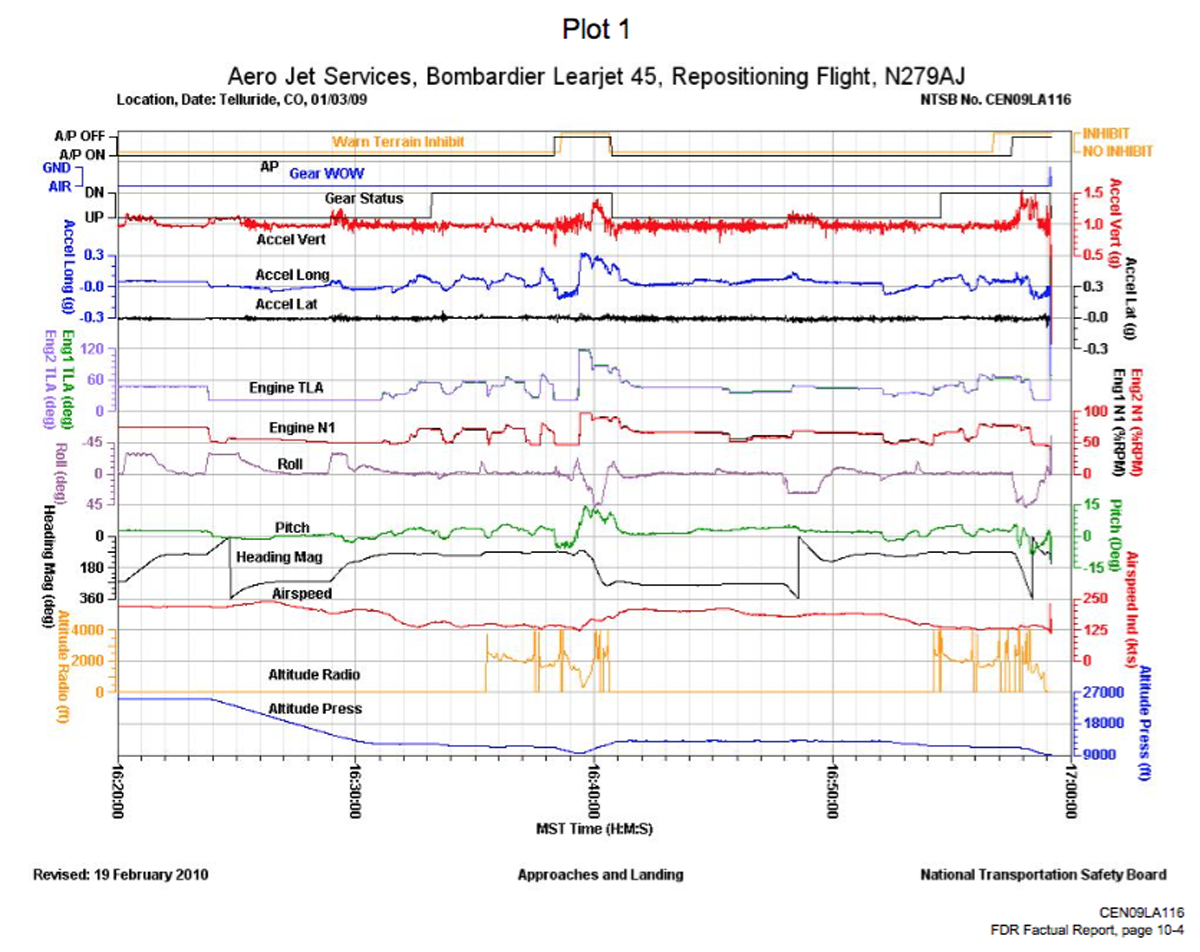
\includegraphics[width=1\textwidth, trim=11mm 0 5mm 2cm, clip=true]{img/ntsb_plot.png}}
	%TODO pojęcie NTSPB
	\caption{Opublikowany w raporcie NTSB wykres wybranych parametrów lotu (3.01.2009)}
	\label{fig:ntsb_plot}
\end{figure}

%todo

\begin{itemize}
	\item serie czasowe jako reprezentacja zbioru danych na osi czasu
	\item kontekstowość w przeglądaniu danych
	\item rola abstrakcji w wizualnej analizie
	\item w przypadku danych pomiarowych - agregacje czasowe
	\item swoboda użytkownika w nawigacji
\end{itemize}


\paragraph{Webowe interfejsy użytkownika}

W ostatnich czasach rosnącą popularność zyskują rozwiązania webowe \cite{dziennik-internautow}, w których graficzny interfejs użytkownika zawarty jest w przeglądarce internetowej \cite{what-is-web-app}.
Warto wspomnieć, że obecnie nowe technologie, takie jak HTML5, CSS3 i modularny JavaScript wypierają wymierające już rozwiązania, takie jak Flash, Silverlight czy aplety Java, które do tej pory były wykorzystywane główne jako narzędzia służące do tworzenia zaawansowanych interfejsów użytkownika \cite{jobs2010thoughts}.


IVA
eksploracja w IVA
Ze względu na ograniczone możliwości ludzkiego mózgu...

\paragraph{Responsywność interfejsu użytkownika}

\paragraph{Architektura klient-serwer}

\paragraph{Cel pracy}

\paragraph{Kontekst pracy}

\subparagraph{Inspiracje}

\subparagraph{Motywacja}

\subparagraph{Prace zwiazane z tematem}

\paragraph{Istniejące rozwiązania}




